\chapter{Resultado das Avaliações}
  
  Essa seção apresenta o resultados das avaliações feitas ao longo do projeto.
  
  \section{Avaliações do protótipo de papel}
     
     Para se realizar a avaliação do protótipo de papel, foi solicitado a 5 usuários com um perfil comum
     e compatível com a proposta do aplicativo (frequentadores de eventos), que realizassem dois cenários para a avaliação:
  
    \begin{itemize}
	\item A - Criar uma notificação com data e hora definidos.
	\item B - Gerenciar (edição e exclusão) suas notificações agendadas.
    \end{itemize}
     
    \noindent
    \textbf{Itens do questionário aplicado}
        
        Abaixo se encontram as perguntas, provenientes do questionário ASQ, que foram utilizadas após a realização
        de cada uma das atividades solicitadas no protótipo de papel:
        
	\begin{enumerate}
	\item No geral, estou satisfeito com a facilidade de completar das atividades neste cenário.
	
	\item No geral, estou satisfeito com a quantidade de tempo que levei para completar as atividades neste cenário.
	
	\item No geral, estou satisfeito com a informação de suporte (ajuda on-line, mensagens, documentação) fornecida
	  enquanto completava as atividades.
	\end{enumerate}
     
	É importante salientar que as questões tinham como opção de resposta de 1 a 7 e a opção “Não se aplica”,
	sendo que 1 significa que o usuário concorda fortemente com o que está sendo perguntado e 7 que o usuário
	discorda fortemente.
  
    \subsection{1ª iteração de avaliação}
        
          A tabela \ref{opnioes1iteracao} descreve o \textit{feedback} dos usuários com os pontos que faltaram na aplicação:
	
  \begin{table}[h]
  \centering
  \begin{tabular}{|m{1.5cm}||m{15cm}|}
    \hline
    \textbf{Usuário} & \textbf{Sentiu falta de:}\\
    
    \hline                               
    1 & 
      \begin{itemize}
	\item Um campo para escolher a cidade do evento na tela de escolher para quando deseja a notificação.
	\item Mensagem de confirmação de exclusão de uma notificação.
      \end{itemize}\\

    \hline                               
    2 & 
      \begin{itemize}
	\item Mensagem de notificação da perda dos dados caso queira voltar para uma tela anterior.
	\item A possibilidade de escolher um intervalo de horário para a notificações, ao invés de um horário fixo.
	\item Ao invés de colocar a mensagem de confirmação do salvamento de uma notificação em uma tela separada, colocar como uma mensagem sobrepondo a mesma tela.
	\item As notificações agendadas poderiam aparecer logo na página inicial.
      \end{itemize}\\
    
    \hline                               
    3 & 
      \begin{itemize}
	\item Uma melhor visualização do campo que exibe as notificações adicionadas.
	\item Lista de notificações agendadas mais centralizada.
	\item Símbolo de “Retirar tema” mais intuitivo.
	\item Caixinha de “Mais temas” na tela de edição.
      \end{itemize}\\
    
    \hline                               
    4 & 
    \begin{itemize}
      \item Especificação que a notificação de horário é referente a notificação.
      \item Melhorar símbolo de “menos” na tela de “Editar notificação”.
    \end{itemize}\\
    
    \hline                               
    5 & 
    \begin{itemize}
      \item Espaço para comentários sobre uma notificação. Ex: Comprar ingresso para a tia Tânia.
    \end{itemize}\\
    
    \hline
  \end{tabular}
  \caption{Opniões dos usuários na 1ª iteração de avaliação.}
  \label{opnioes1iteracao}
  \end{table}
  
  Na figura \ref{resposta_asq_1iteracao} se encontram as respostas ao questionário ASQ pelos cinco usuários avaliados.

  \begin{figure}[!htb]
  \centering
  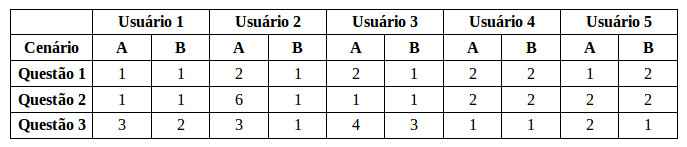
\includegraphics[scale=0.6]{figuras/nota1avaliacao.jpg}
  \caption{Resposta dos usuários ao questionário ASQ na primeira avaliação do protótipo de papel}
  \label{resposta_asq_1iteracao}
  \end{figure}
    
    \pagebreak
    \subsection{2ª iteração de avaliação}
	
	  A tabela \ref{opnioes2iteracao} descreve o \textit{feedback} dos usuários com os pontos que faltaram na aplicação:
	
  \begin{table}[h]
  \centering
  \begin{tabular}{|m{1.5cm}||m{15cm}|}
    \hline
    \textbf{Usuário} & \textbf{Sentiu falta de:}\\
    
    \hline                               
    1 & 
      \begin{itemize}
	\item Deixar as informações na tela mais divididas.
	\item Uma opção ao usuário de registro.
      \end{itemize}\\

    \hline                               
    2 & 
      \begin{itemize}
	\item Cancelar a edição da notificação.
	\item Fazer confirmação de alterado com sucesso.
      \end{itemize}\\
    
    \hline                               
    3 & 
      \begin{itemize}
	\item Programar para aviso prévio (não no dia).
	\item A cidade ser a primeira a ser selecionada para limitação do seventos.
      \end{itemize}\\
    
    \hline                               
    4 & 
    \begin{itemize}
      \item Deixar o "Não" destacado da opção de excluir notificação.
    \end{itemize}\\
    
    \hline                               
    5 & 
    \begin{itemize}
      \item Não há sugestões.
    \end{itemize}\\
    
    \hline
  \end{tabular}
  \caption{Opniões dos usuários na 2ª iteração de avaliação.}
  \label{opnioes2iteracao}
  \end{table}
  
  
  
  Na figura \ref{resposta_asq_2iteracao} se encontram as respostas ao questionário ASQ pelos cinco usuários avaliados.

  
  
  \begin{figure}[!htb]
  \centering
  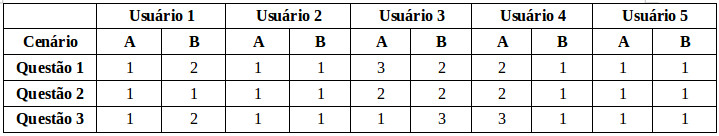
\includegraphics[scale=0.7]{figuras/nota2avaliacao.jpg}
  \caption{Resposta dos usuários ao questionário ASQ na segunda avaliação do protótipo de papel}
  \label{resposta_asq_2iteracao}
  \end{figure}
  
  \pagebreak
  \subsection{Análise dos resultados da avaliação do protótipo de papel}
    
    \subsubsection{1ª iteração}
      
      Na primeira iteração, o objetivo primário de levantar requisitos foi cumprido com louvor.
      Todas as colocações levantadas pelos usuários foram analisadas pela equipe e aceitas quase que totalmente.
      
      A partir da observação do usuário foi possível analisar também as metas definidas para a iteração de avaliação.
      
      Com a aplicação do questionário ASQ, foi possível avaliar a facilidade de uso do aplicativo, a reação do usuário 
      com o tempo gasto para realizar as tarefas e satisfação do usuário com o suporte do aplicativo, mesmo na primeira
      fase de prototipação. Com esses dados é possível perceber a evolução do protótipo em relação à percepção do usuário.
      
    \subsubsection{2ª iteração}
    
      Na segunda iteração poucas colocações foram levantadas pelos usuários avaliados, mas as que foram levantadas também foram
      analisadas pela equipe e consideradas para a construção do protótipo de mais alta fidelidade.
      
      Não foi feita outra iteração de avaliação do protótipo de papel porque nesta iteração surgiram poucas mudanças,
      evidenciando a estabilização do protótipo de papel.
      
      Nessa iteração também foram coletadas as respostas ao questionário ASQ. A análise dos dados se encontra logo abaixo.
    
    \subsubsection{Análise geral}
    
      O registro das respostas dos usuários ao questionário ASQ permitiu ver a evolução dos cenários nas versões do 
      protótipo de papel. Foi tirada a média das respostas dos cinco usuários avaliados para cada iteração de avaliação
      e o resultado se encontra na figura \ref{evolucao_prototipo_papel_ASQ}.
      
      \begin{figure}[!htpb]
	\centering
	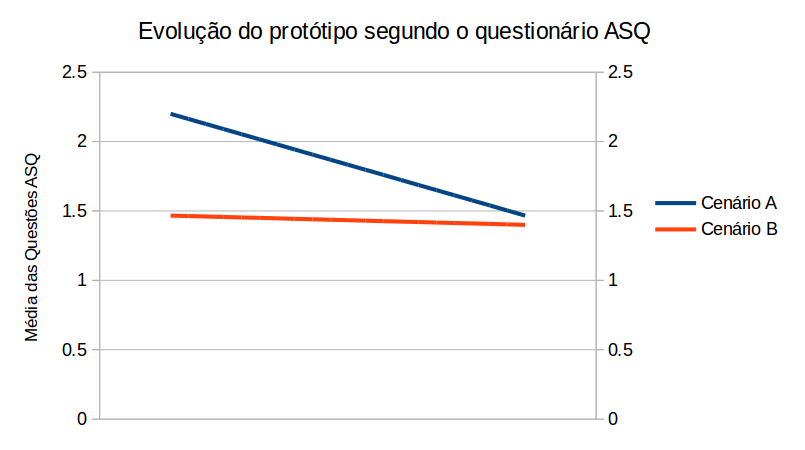
\includegraphics[scale=0.35]{editaveis/figuras/evolucao_prototipo_papel_ASQ}
	\caption[Evolução do protótipo de papel, segundo o questionário ASQ]
	  {Evolução do protótipo de papel, segundo o questionário ASQ.}
	\label{evolucao_prototipo_papel_ASQ}
      \end{figure}
      
      Pelo gráfico apresentado na figura \ref{evolucao_prototipo_papel_ASQ}, é possível ver que houve uma evolução significativa
      no protótipo no cenário A, enquanto no cenário B houveram poucas mudanças. No geral, percebe-se que o protótipo evoluiu
      bem na percepção dos usuários, uma vez que, segundo a pontuação proposta pelo ASQ, quanto mais próximo de 1 estiver
      a pontuação das respostas às perguntas, mais o usuário concorda e está satisfeito com o cenário.
      
  \section{Avaliações do protótipo de alta fidelidade}
    
    Essa seção descreve os resultados obtidos com a avaliação do protótipo de alta fidelidade.
    
    \subsection{1ª iteração de avaliação}
    
      Logo abaixo são apresentados os resultados da primeira iteração de avaliação do protótipo.
      
      \begin{itemize}
       \item \textbf{Descrição e metodologia do roteiro da avaliação}
       
       \item \textbf{Comportamento dos usuários}
       
       \item \textbf{Resumo das entrevistas}
       
       \item \textbf{Problemas de usabilidade identificados}
       
       \item \textbf{Paradas críticas}
       
       \item \textbf{Plano de correção}
      \end{itemize}
